\documentclass[ignorenonframetext,]{beamer}
\setbeamertemplate{caption}[numbered]
\setbeamertemplate{caption label separator}{: }
\setbeamercolor{caption name}{fg=normal text.fg}
\beamertemplatenavigationsymbolsempty
\usepackage{lmodern}
\usepackage{amssymb,amsmath}
\usepackage{ifxetex,ifluatex}
\usepackage{fixltx2e} % provides \textsubscript
\ifnum 0\ifxetex 1\fi\ifluatex 1\fi=0 % if pdftex
  \usepackage[T1]{fontenc}
  \usepackage[utf8]{inputenc}
\else % if luatex or xelatex
  \ifxetex
    \usepackage{mathspec}
  \else
    \usepackage{fontspec}
  \fi
  \defaultfontfeatures{Ligatures=TeX,Scale=MatchLowercase}
\fi
\usetheme[]{CambridgeUS}
\usecolortheme{beaver}
\usefonttheme{structurebold}
% use upquote if available, for straight quotes in verbatim environments
\IfFileExists{upquote.sty}{\usepackage{upquote}}{}
% use microtype if available
\IfFileExists{microtype.sty}{%
\usepackage{microtype}
\UseMicrotypeSet[protrusion]{basicmath} % disable protrusion for tt fonts
}{}
\newif\ifbibliography
\hypersetup{
            pdftitle={Javascript Bibliotheken nutzen},
            pdfauthor={Jan-Philipp Kolb},
            pdfborder={0 0 0},
            breaklinks=true}
\urlstyle{same}  % don't use monospace font for urls
\usepackage{color}
\usepackage{fancyvrb}
\newcommand{\VerbBar}{|}
\newcommand{\VERB}{\Verb[commandchars=\\\{\}]}
\DefineVerbatimEnvironment{Highlighting}{Verbatim}{commandchars=\\\{\}}
% Add ',fontsize=\small' for more characters per line
\usepackage{framed}
\definecolor{shadecolor}{RGB}{248,248,248}
\newenvironment{Shaded}{\begin{snugshade}}{\end{snugshade}}
\newcommand{\KeywordTok}[1]{\textcolor[rgb]{0.13,0.29,0.53}{\textbf{#1}}}
\newcommand{\DataTypeTok}[1]{\textcolor[rgb]{0.13,0.29,0.53}{#1}}
\newcommand{\DecValTok}[1]{\textcolor[rgb]{0.00,0.00,0.81}{#1}}
\newcommand{\BaseNTok}[1]{\textcolor[rgb]{0.00,0.00,0.81}{#1}}
\newcommand{\FloatTok}[1]{\textcolor[rgb]{0.00,0.00,0.81}{#1}}
\newcommand{\ConstantTok}[1]{\textcolor[rgb]{0.00,0.00,0.00}{#1}}
\newcommand{\CharTok}[1]{\textcolor[rgb]{0.31,0.60,0.02}{#1}}
\newcommand{\SpecialCharTok}[1]{\textcolor[rgb]{0.00,0.00,0.00}{#1}}
\newcommand{\StringTok}[1]{\textcolor[rgb]{0.31,0.60,0.02}{#1}}
\newcommand{\VerbatimStringTok}[1]{\textcolor[rgb]{0.31,0.60,0.02}{#1}}
\newcommand{\SpecialStringTok}[1]{\textcolor[rgb]{0.31,0.60,0.02}{#1}}
\newcommand{\ImportTok}[1]{#1}
\newcommand{\CommentTok}[1]{\textcolor[rgb]{0.56,0.35,0.01}{\textit{#1}}}
\newcommand{\DocumentationTok}[1]{\textcolor[rgb]{0.56,0.35,0.01}{\textbf{\textit{#1}}}}
\newcommand{\AnnotationTok}[1]{\textcolor[rgb]{0.56,0.35,0.01}{\textbf{\textit{#1}}}}
\newcommand{\CommentVarTok}[1]{\textcolor[rgb]{0.56,0.35,0.01}{\textbf{\textit{#1}}}}
\newcommand{\OtherTok}[1]{\textcolor[rgb]{0.56,0.35,0.01}{#1}}
\newcommand{\FunctionTok}[1]{\textcolor[rgb]{0.00,0.00,0.00}{#1}}
\newcommand{\VariableTok}[1]{\textcolor[rgb]{0.00,0.00,0.00}{#1}}
\newcommand{\ControlFlowTok}[1]{\textcolor[rgb]{0.13,0.29,0.53}{\textbf{#1}}}
\newcommand{\OperatorTok}[1]{\textcolor[rgb]{0.81,0.36,0.00}{\textbf{#1}}}
\newcommand{\BuiltInTok}[1]{#1}
\newcommand{\ExtensionTok}[1]{#1}
\newcommand{\PreprocessorTok}[1]{\textcolor[rgb]{0.56,0.35,0.01}{\textit{#1}}}
\newcommand{\AttributeTok}[1]{\textcolor[rgb]{0.77,0.63,0.00}{#1}}
\newcommand{\RegionMarkerTok}[1]{#1}
\newcommand{\InformationTok}[1]{\textcolor[rgb]{0.56,0.35,0.01}{\textbf{\textit{#1}}}}
\newcommand{\WarningTok}[1]{\textcolor[rgb]{0.56,0.35,0.01}{\textbf{\textit{#1}}}}
\newcommand{\AlertTok}[1]{\textcolor[rgb]{0.94,0.16,0.16}{#1}}
\newcommand{\ErrorTok}[1]{\textcolor[rgb]{0.64,0.00,0.00}{\textbf{#1}}}
\newcommand{\NormalTok}[1]{#1}
\usepackage{longtable,booktabs}
\usepackage{caption}
% These lines are needed to make table captions work with longtable:
\makeatletter
\def\fnum@table{\tablename~\thetable}
\makeatother
\usepackage{graphicx,grffile}
\makeatletter
\def\maxwidth{\ifdim\Gin@nat@width>\linewidth\linewidth\else\Gin@nat@width\fi}
\def\maxheight{\ifdim\Gin@nat@height>\textheight0.8\textheight\else\Gin@nat@height\fi}
\makeatother
% Scale images if necessary, so that they will not overflow the page
% margins by default, and it is still possible to overwrite the defaults
% using explicit options in \includegraphics[width, height, ...]{}
\setkeys{Gin}{width=\maxwidth,height=\maxheight,keepaspectratio}

% Prevent slide breaks in the middle of a paragraph:
\widowpenalties 1 10000
\raggedbottom

\AtBeginPart{
  \let\insertpartnumber\relax
  \let\partname\relax
  \frame{\partpage}
}
\AtBeginSection{
  \ifbibliography
  \else
    \let\insertsectionnumber\relax
    \let\sectionname\relax
    \frame{\sectionpage}
  \fi
}
\AtBeginSubsection{
  \let\insertsubsectionnumber\relax
  \let\subsectionname\relax
  \frame{\subsectionpage}
}

\setlength{\parindent}{0pt}
\setlength{\parskip}{6pt plus 2pt minus 1pt}
\setlength{\emergencystretch}{3em}  % prevent overfull lines
\providecommand{\tightlist}{%
  \setlength{\itemsep}{0pt}\setlength{\parskip}{0pt}}
\setcounter{secnumdepth}{0}

\title{Javascript Bibliotheken nutzen}
\author{Jan-Philipp Kolb}
\date{23 Oktober 2018}

\begin{document}
\frame{\titlepage}

\begin{frame}[fragile]{Beispiel zu Campingplätzen}

\begin{itemize}
\tightlist
\item
  Die Daten stammen von:
\end{itemize}

\url{http://www.openstreetmap.de/}

\begin{itemize}
\tightlist
\item
  Dabei wird die Overpass API genutzt:
\end{itemize}

\url{http://wiki.openstreetmap.org/wiki/Overpass_API}

\begin{Shaded}
\begin{Highlighting}[]
\NormalTok{url <-}\StringTok{ "https://raw.githubusercontent.com/Japhilko/}
\StringTok{GeoData/master/2015/data/CampSites_Germany.csv"}
\end{Highlighting}
\end{Shaded}

\begin{Shaded}
\begin{Highlighting}[]
\NormalTok{CampSites <-}\StringTok{ }\KeywordTok{read.csv}\NormalTok{(url)}
\end{Highlighting}
\end{Shaded}

\end{frame}

\begin{frame}{Überblick über Daten zu Campingplätzen}

\begin{longtable}[]{@{}rlll@{}}
\toprule
X & name & tourism & website\tabularnewline
\midrule
\endhead
1 & Campingplatz Winkelbachtal & camp\_site &
\url{http://www.gruibingen.de/campingplatz.html}\tabularnewline
2 & Radler-Zeltplatz & camp\_site & NA\tabularnewline
3 & Campingplatz des Naturfreundehauses & camp\_site & NA\tabularnewline
4 & Campingplatz Am Aichstruter Stausee & camp\_site & NA\tabularnewline
5 & NA & camp\_site & NA\tabularnewline
6 & Kandern & camp\_site & NA\tabularnewline
7 & Campingplatz Baiersbronn-Obertal & camp\_site & NA\tabularnewline
8 & Campingplatz Schwabenmühle & camp\_site & NA\tabularnewline
\bottomrule
\end{longtable}

\end{frame}

\begin{frame}[fragile]{Notwendige Pakete}

\href{https://cran.r-project.org/web/packages/magrittr/index.html}{magrittr}
- für den Pipe Operator in R:

\begin{Shaded}
\begin{Highlighting}[]
\KeywordTok{library}\NormalTok{(}\StringTok{"magrittr"}\NormalTok{)}
\end{Highlighting}
\end{Shaded}

\href{https://rstudio.github.io/leaflet/}{leaflet} - um interaktive
Karten mit der JavaScript Bibliothek `Leaflet' zu erzeugen

\begin{Shaded}
\begin{Highlighting}[]
\KeywordTok{library}\NormalTok{(}\StringTok{"leaflet"}\NormalTok{)}
\end{Highlighting}
\end{Shaded}

\end{frame}

\begin{frame}[fragile]{Eine erste interaktive Karte}

\begin{Shaded}
\begin{Highlighting}[]
\KeywordTok{leaflet}\NormalTok{()}\OperatorTok
\StringTok{  }\KeywordTok{addTiles}\NormalTok{()}
\end{Highlighting}
\end{Shaded}

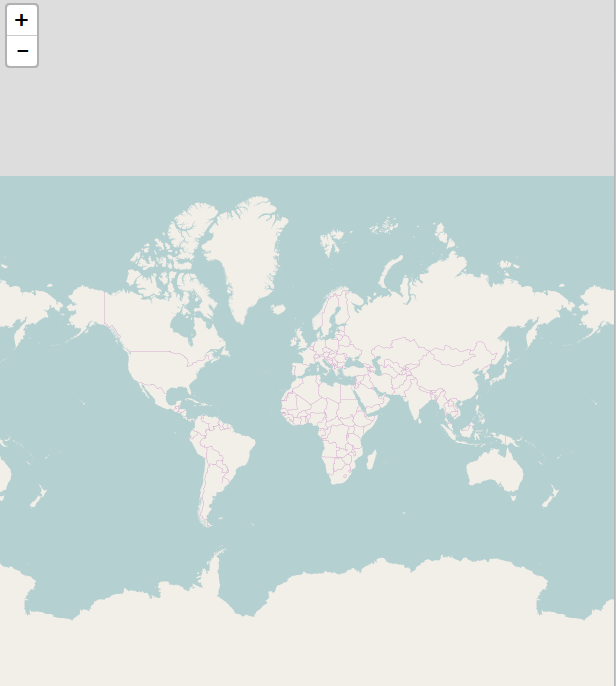
\includegraphics{figure/FirstLeaflet.PNG}

\end{frame}

\begin{frame}[fragile]{Auf eine Stadt zoomen}

\begin{Shaded}
\begin{Highlighting}[]
\KeywordTok{leaflet}\NormalTok{() }\OperatorTok
\StringTok{  }\KeywordTok{addTiles}\NormalTok{() }\OperatorTok
\StringTok{  }\KeywordTok{addMarkers}\NormalTok{(}\DataTypeTok{lng=}\FloatTok{8.456597}\NormalTok{, }\DataTypeTok{lat=}\FloatTok{49.48738}\NormalTok{,}
             \DataTypeTok{popup=}\StringTok{"Wo wir sind"}\NormalTok{)}
\end{Highlighting}
\end{Shaded}

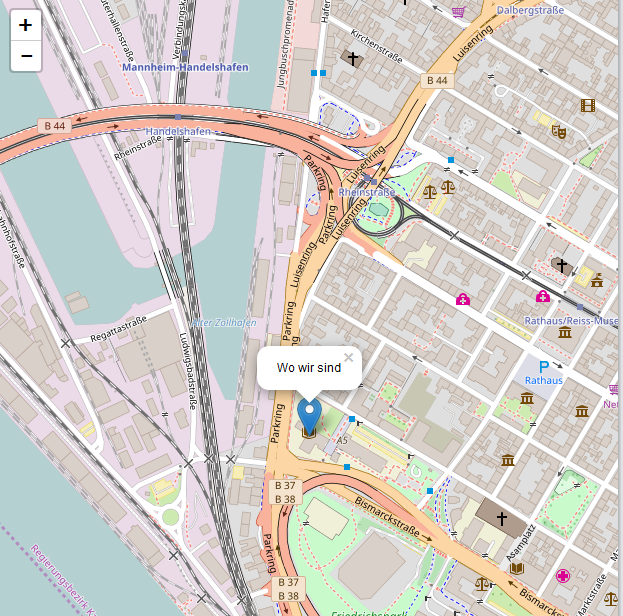
\includegraphics{figure/leafletMZESMA.PNG}

\end{frame}

\begin{frame}[fragile]{Eine interaktive Karte}

\begin{Shaded}
\begin{Highlighting}[]
\NormalTok{m <-}\StringTok{ }\KeywordTok{leaflet}\NormalTok{() }\OperatorTok
\StringTok{  }\KeywordTok{addTiles}\NormalTok{() }\OperatorTok\StringTok{  }
\StringTok{  }\KeywordTok{addMarkers}\NormalTok{(}\DataTypeTok{lng=}\NormalTok{CampSites}\OperatorTok{$}\NormalTok{lon, }
             \DataTypeTok{lat=}\NormalTok{CampSites}\OperatorTok{$}\NormalTok{lat, }
             \DataTypeTok{popup=}\NormalTok{CampSites}\OperatorTok{$}\NormalTok{name)}
\NormalTok{m}
\end{Highlighting}
\end{Shaded}

\end{frame}

\begin{frame}[fragile]{\href{https://rstudio.github.io/leaflet/basemaps.html}{Stamen
als Hintergrundkarte}}

\begin{Shaded}
\begin{Highlighting}[]
\NormalTok{m }\OperatorTok\StringTok{ }\KeywordTok{addProviderTiles}\NormalTok{(}\StringTok{"Stamen.Toner"}\NormalTok{)}
\end{Highlighting}
\end{Shaded}

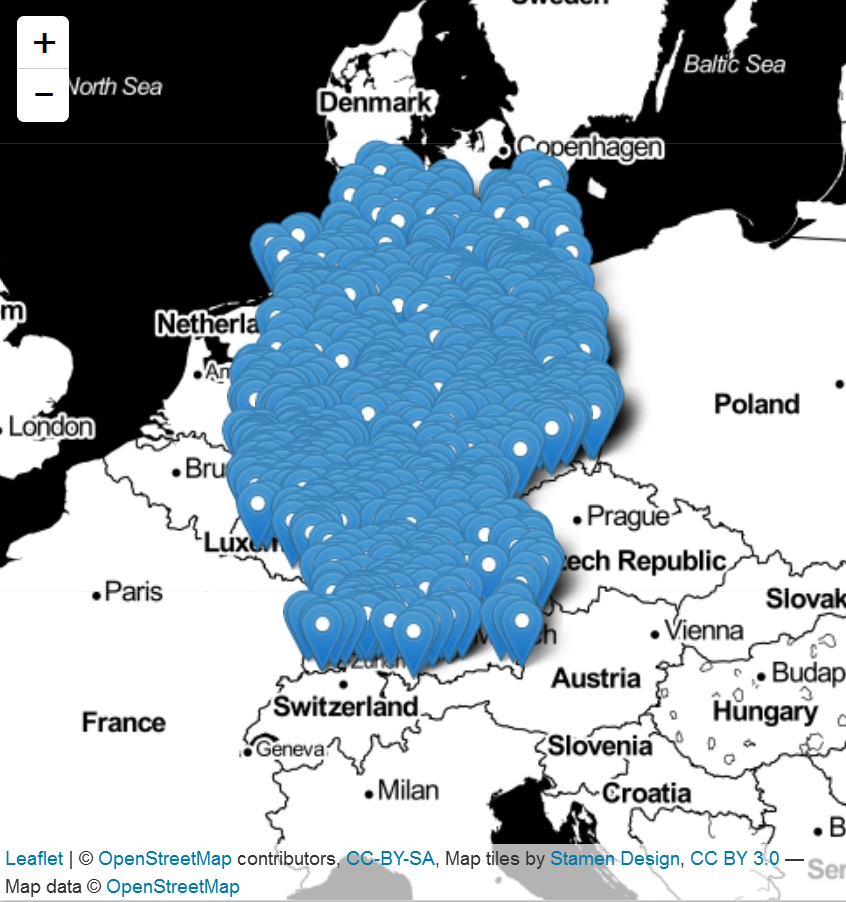
\includegraphics{figure/InteractiveStamen.PNG}

\end{frame}

\begin{frame}[fragile]{CartoDB als Hintergrund}

\begin{Shaded}
\begin{Highlighting}[]
\NormalTok{m }\OperatorTok\StringTok{ }\KeywordTok{addProviderTiles}\NormalTok{(}\StringTok{"CartoDB.Positron"}\NormalTok{)}
\end{Highlighting}
\end{Shaded}

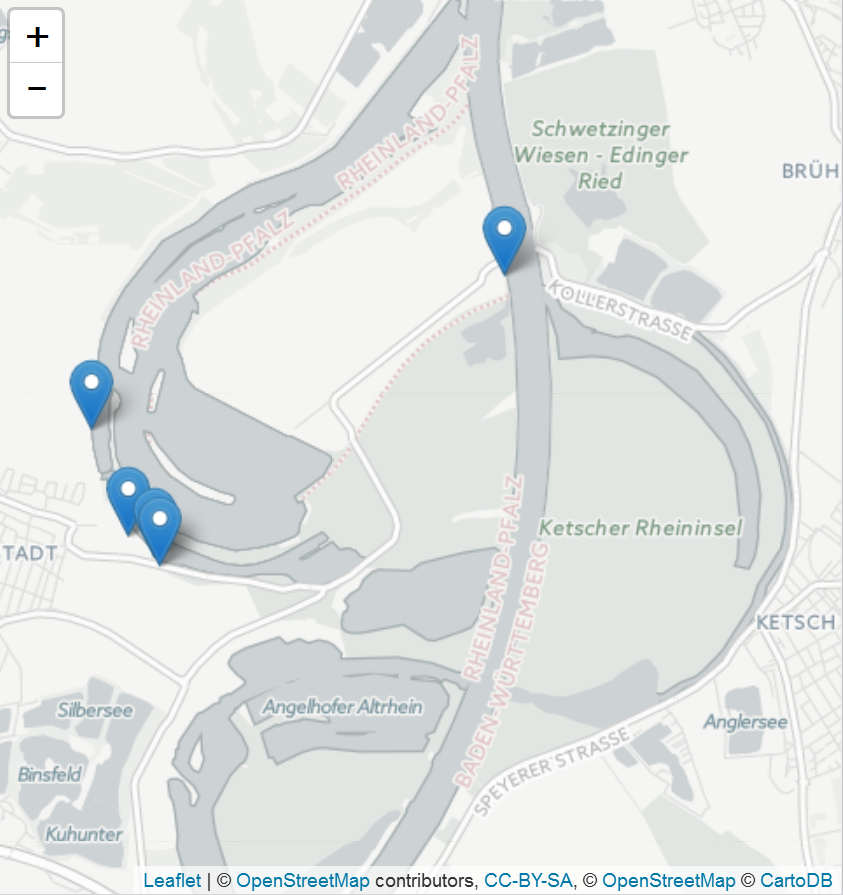
\includegraphics{figure/CartoDBInteractive.PNG}

\begin{itemize}
\item
  \href{https://carto.com/attribution}{CartoDB}
\item
  \href{https://www.mapbox.com/help/how-web-maps-work/}{Info zu Map
  Tiles}
\end{itemize}

\end{frame}

\begin{frame}[fragile]{\href{http://leaflet-extras.github.io/leaflet-providers/preview/index.html}{Mehr
Hintergründe}}

\begin{Shaded}
\begin{Highlighting}[]
\NormalTok{m }\OperatorTok\StringTok{ }\KeywordTok{addProviderTiles}\NormalTok{(}\StringTok{"NASAGIBS.ViirsEarthAtNight2012"}\NormalTok{)}
\end{Highlighting}
\end{Shaded}

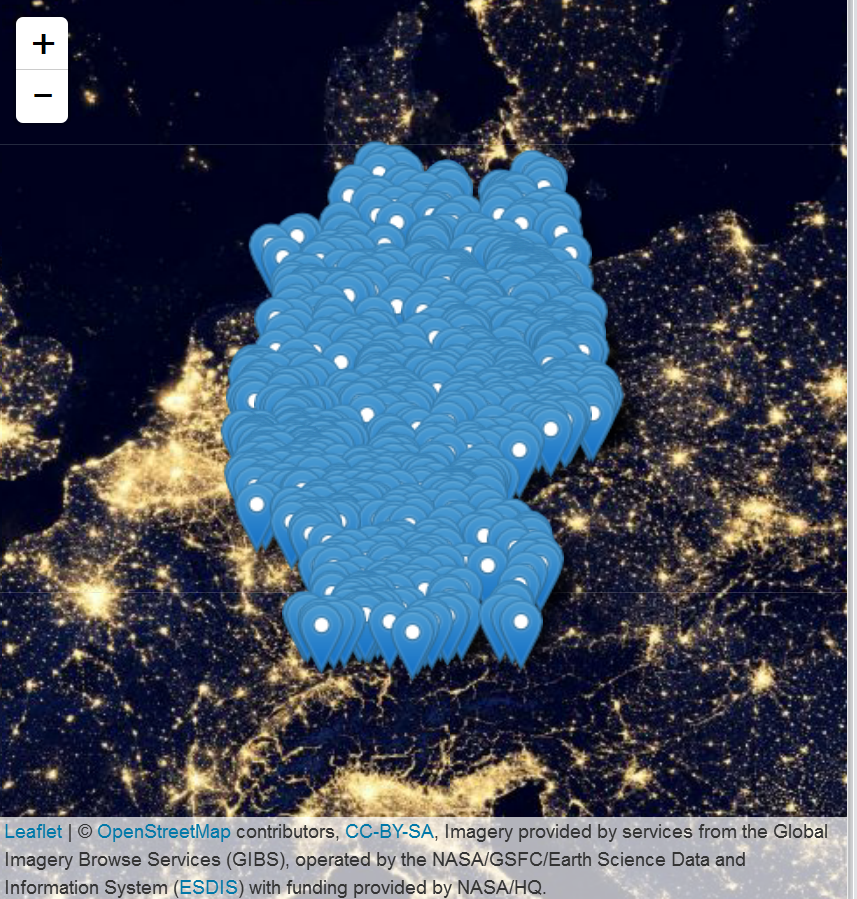
\includegraphics{figure/LightsInteractive.PNG}

\end{frame}

\begin{frame}[fragile]{Mehr Informationen hinzufügen}

\begin{Shaded}
\begin{Highlighting}[]
\NormalTok{popupInfo <-}\StringTok{ }\KeywordTok{paste}\NormalTok{(CampSites}\OperatorTok{$}\NormalTok{name,}\StringTok{"}\CharTok{\textbackslash{}n}\StringTok{"}\NormalTok{,CampSites}\OperatorTok{$}\NormalTok{website)}
\end{Highlighting}
\end{Shaded}

\begin{Shaded}
\begin{Highlighting}[]
\NormalTok{m <-}\StringTok{ }\KeywordTok{leaflet}\NormalTok{() }\OperatorTok
\StringTok{  }\KeywordTok{addTiles}\NormalTok{() }\OperatorTok\StringTok{  }\CommentTok{# Add default OpenStreetMap map tiles}
\StringTok{  }\KeywordTok{addMarkers}\NormalTok{(}\DataTypeTok{lng=}\NormalTok{CampSites}\OperatorTok{$}\NormalTok{lon, }
             \DataTypeTok{lat=}\NormalTok{CampSites}\OperatorTok{$}\NormalTok{lat, }
             \DataTypeTok{popup=}\NormalTok{popupInfo)}
\NormalTok{m}
\end{Highlighting}
\end{Shaded}

Das Ergebnis ist hier:

\url{http://rpubs.com/Japhilko82/CampSitesHL}

\end{frame}

\begin{frame}{Die resultierende Karte}

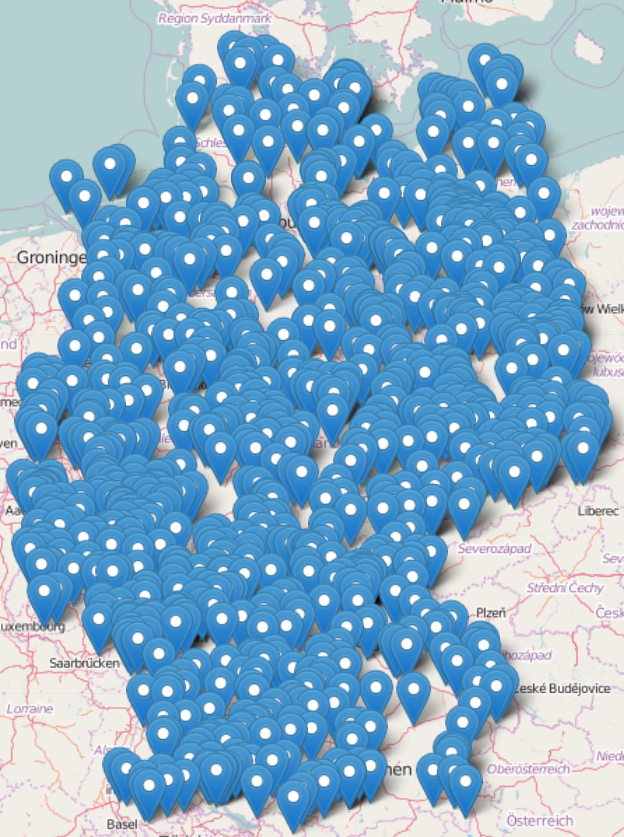
\includegraphics{figure/Germany_Campsites.PNG}

\end{frame}

\begin{frame}{Popups in einer interactiven Karte}

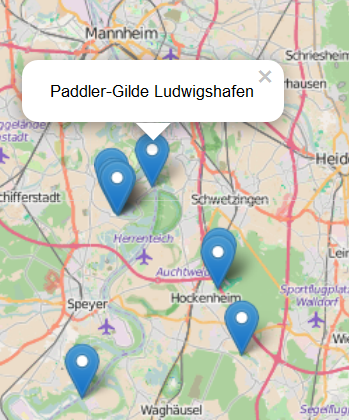
\includegraphics{figure/Camping_Mannheim.PNG}

Ich hab die Ergebnisse hochgeladen:

\url{http://rpubs.com/Japhilko82/Campsites}

\end{frame}

\begin{frame}{Wie man auf Rpubs publizieren kann}

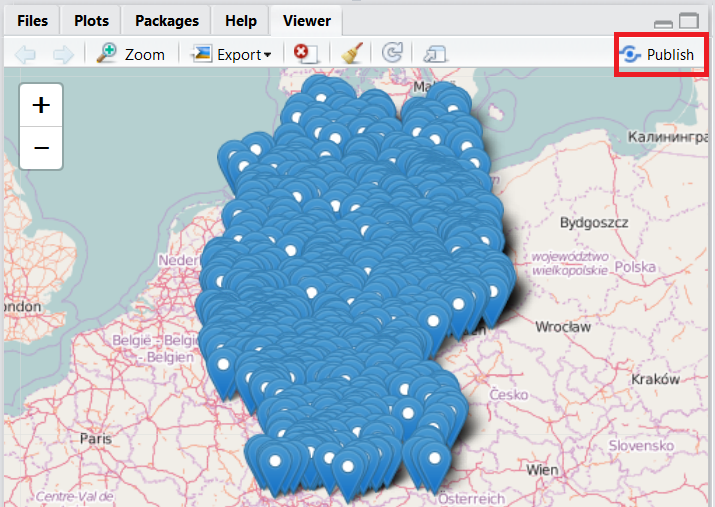
\includegraphics{figure/PublishCampSitesGermany.PNG}

\end{frame}

\begin{frame}[fragile]{Ein weiteres Beispiel - Weltkulturerbe}

\begin{Shaded}
\begin{Highlighting}[]
\NormalTok{url <-}\StringTok{ "https://raw.githubusercontent.com/Japhilko/}
\StringTok{GeoData/master/2015/data/whcSites.csv"}

\NormalTok{whcSites <-}\StringTok{ }\KeywordTok{read.csv}\NormalTok{(url) }
\end{Highlighting}
\end{Shaded}

\end{frame}

\begin{frame}[fragile]{Eine interaktive Karte erstellen}

\begin{Shaded}
\begin{Highlighting}[]
\NormalTok{m <-}\StringTok{ }\KeywordTok{leaflet}\NormalTok{() }\OperatorTok
\StringTok{  }\KeywordTok{addTiles}\NormalTok{() }\OperatorTok\StringTok{  }\CommentTok{# Add default OpenStreetMap map tiles}
\StringTok{  }\KeywordTok{addMarkers}\NormalTok{(}\DataTypeTok{lng=}\NormalTok{whcSites}\OperatorTok{$}\NormalTok{lon, }
             \DataTypeTok{lat=}\NormalTok{whcSites}\OperatorTok{$}\NormalTok{lat, }
             \DataTypeTok{popup=}\NormalTok{whcSites}\OperatorTok{$}\NormalTok{name_en)}
\NormalTok{m}
\end{Highlighting}
\end{Shaded}

\end{frame}

\begin{frame}{Die Karte zeigen}

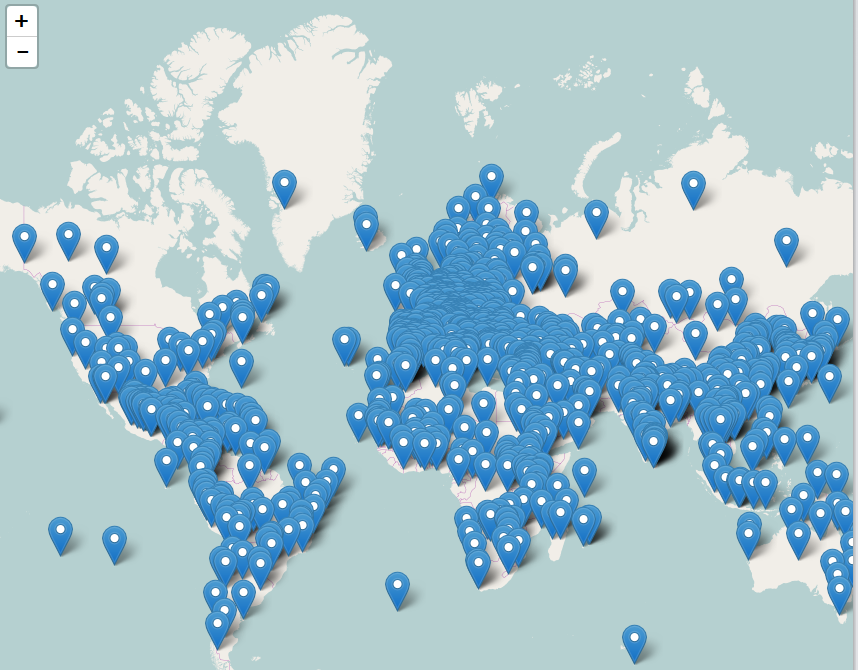
\includegraphics{figure/WHCPopUps.PNG}

\end{frame}

\begin{frame}[fragile]{Farbe hinzu}

\begin{Shaded}
\begin{Highlighting}[]
\NormalTok{whcSites}\OperatorTok{$}\NormalTok{color <-}\StringTok{ "red"}
\NormalTok{whcSites}\OperatorTok{$}\NormalTok{color[whcSites}\OperatorTok{$}\NormalTok{category}\OperatorTok{==}\StringTok{"Cultural"}\NormalTok{] <-}\StringTok{ "blue"}
\NormalTok{whcSites}\OperatorTok{$}\NormalTok{color[whcSites}\OperatorTok{$}\NormalTok{category}\OperatorTok{==}\StringTok{"Mixed"}\NormalTok{] <-}\StringTok{ "orange"}
\end{Highlighting}
\end{Shaded}

\end{frame}

\begin{frame}[fragile]{Eine Karte mit Farbe erzeugen}

\begin{Shaded}
\begin{Highlighting}[]
\NormalTok{m1 <-}\StringTok{ }\KeywordTok{leaflet}\NormalTok{() }\OperatorTok
\StringTok{  }\KeywordTok{addTiles}\NormalTok{() }\OperatorTok\StringTok{  }
\StringTok{  }\KeywordTok{addCircles}\NormalTok{(}\DataTypeTok{lng=}\NormalTok{whcSites}\OperatorTok{$}\NormalTok{lon, }
             \DataTypeTok{lat=}\NormalTok{whcSites}\OperatorTok{$}\NormalTok{lat, }
             \DataTypeTok{popup=}\NormalTok{whcSites}\OperatorTok{$}\NormalTok{name_en,}
             \DataTypeTok{color=}\NormalTok{whcSites}\OperatorTok{$}\NormalTok{color)}
\NormalTok{m1}
\end{Highlighting}
\end{Shaded}

\end{frame}

\begin{frame}{Die Karte zeigen}

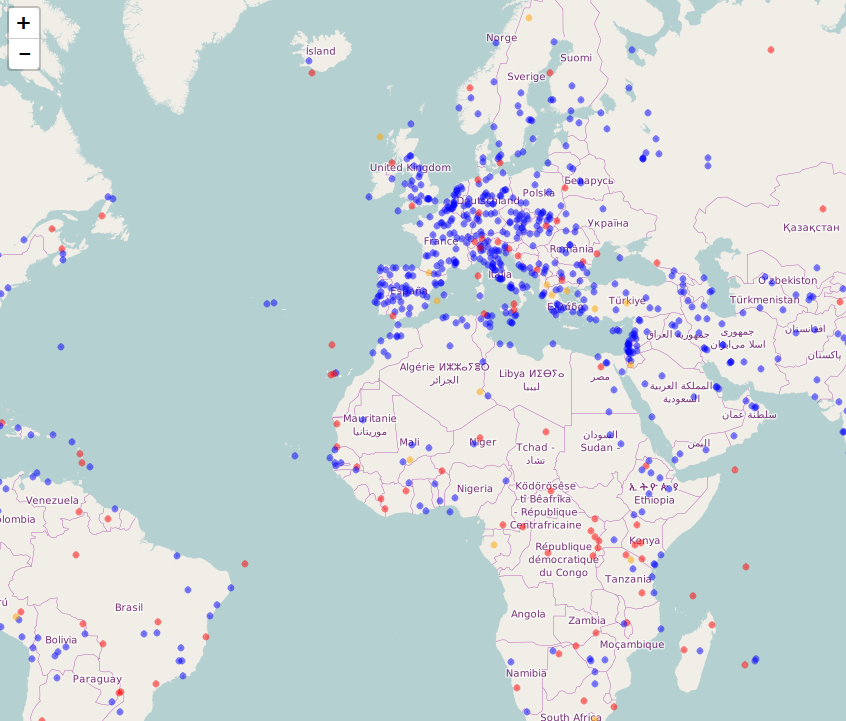
\includegraphics{figure/WHCcircles.PNG}

\end{frame}

\begin{frame}{\href{http://www.r-bloggers.com/interactive-mapping-with-leaflet-in-r-2/}{Die
Karte abspeichern}}

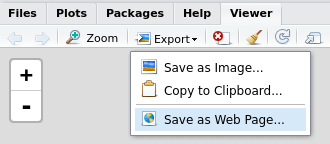
\includegraphics{figure/snapshot2.png}

\end{frame}

\begin{frame}[fragile]{Das Paket \texttt{mapview}}

\begin{Shaded}
\begin{Highlighting}[]
\KeywordTok{load}\NormalTok{(}\StringTok{"../data/spatsamp_68239.RData"}\NormalTok{)}
\end{Highlighting}
\end{Shaded}

\begin{Shaded}
\begin{Highlighting}[]
\KeywordTok{library}\NormalTok{(mapview)}
\KeywordTok{mapview}\NormalTok{(spatsamp)}
\end{Highlighting}
\end{Shaded}

\end{frame}

\begin{frame}[fragile]{Das Paket \texttt{leaflet}}

\begin{Shaded}
\begin{Highlighting}[]
\KeywordTok{library}\NormalTok{(}\StringTok{"tmaptools"}\NormalTok{)}
\NormalTok{gc_tma <-}\StringTok{ }\KeywordTok{geocode_OSM}\NormalTok{(}\StringTok{"Mannheim, GESIS"}\NormalTok{)}
\end{Highlighting}
\end{Shaded}

\begin{Shaded}
\begin{Highlighting}[]
\KeywordTok{library}\NormalTok{(leaflet)}
\KeywordTok{library}\NormalTok{(magrittr)}
\NormalTok{m <-}\StringTok{ }\KeywordTok{leaflet}\NormalTok{() }\OperatorTok
\KeywordTok{addTiles}\NormalTok{() }\OperatorTok
\KeywordTok{addMarkers}\NormalTok{(}\DataTypeTok{lng=}\FloatTok{8.463061}\NormalTok{ , }\DataTypeTok{lat=}\FloatTok{49.485736}\NormalTok{ , }\DataTypeTok{popup=}\StringTok{"GESIS Mannheim"}\NormalTok{)}
\NormalTok{m}
\end{Highlighting}
\end{Shaded}

\end{frame}

\begin{frame}[fragile]{Das Paket \texttt{geojsonR}}

\begin{itemize}
\tightlist
\item
  JavaScript Object Notation
\end{itemize}

\begin{Shaded}
\begin{Highlighting}[]
\KeywordTok{install.packages}\NormalTok{(}\StringTok{"geojsonR"}\NormalTok{)}
\KeywordTok{citation}\NormalTok{(}\StringTok{"geojsonR"}\NormalTok{)}
\end{Highlighting}
\end{Shaded}

\end{frame}

\begin{frame}[fragile]{Wo bekomme ich ein geojson}

\begin{itemize}
\tightlist
\item
  Ein
  \href{https://wiki.openstreetmap.org/wiki/Map_Features}{\textbf{OSM
  map feature}} heraus suchen
\item
  z.B. \texttt{key=highway}, \texttt{value=bus\_stop}
\item
  Auf \href{https://overpass-turbo.eu/}{\textbf{Overpass Turbo}} gehen
  und das Objekt herunterladen
\end{itemize}

\begin{Shaded}
\begin{Highlighting}[]
\NormalTok{bus_stops <-}\StringTok{ }\NormalTok{geojsonio}\OperatorTok{::}\KeywordTok{geojson_read}\NormalTok{(}\StringTok{"../data/Amsterdam_bus_stop.geojson"}\NormalTok{,}
  \DataTypeTok{what =} \StringTok{"sp"}\NormalTok{)}
\end{Highlighting}
\end{Shaded}

\end{frame}

\begin{frame}[fragile]{Die Punkte plotten}

\begin{Shaded}
\begin{Highlighting}[]
\NormalTok{sp}\OperatorTok{::}\KeywordTok{plot}\NormalTok{(bus_stops)}
\end{Highlighting}
\end{Shaded}

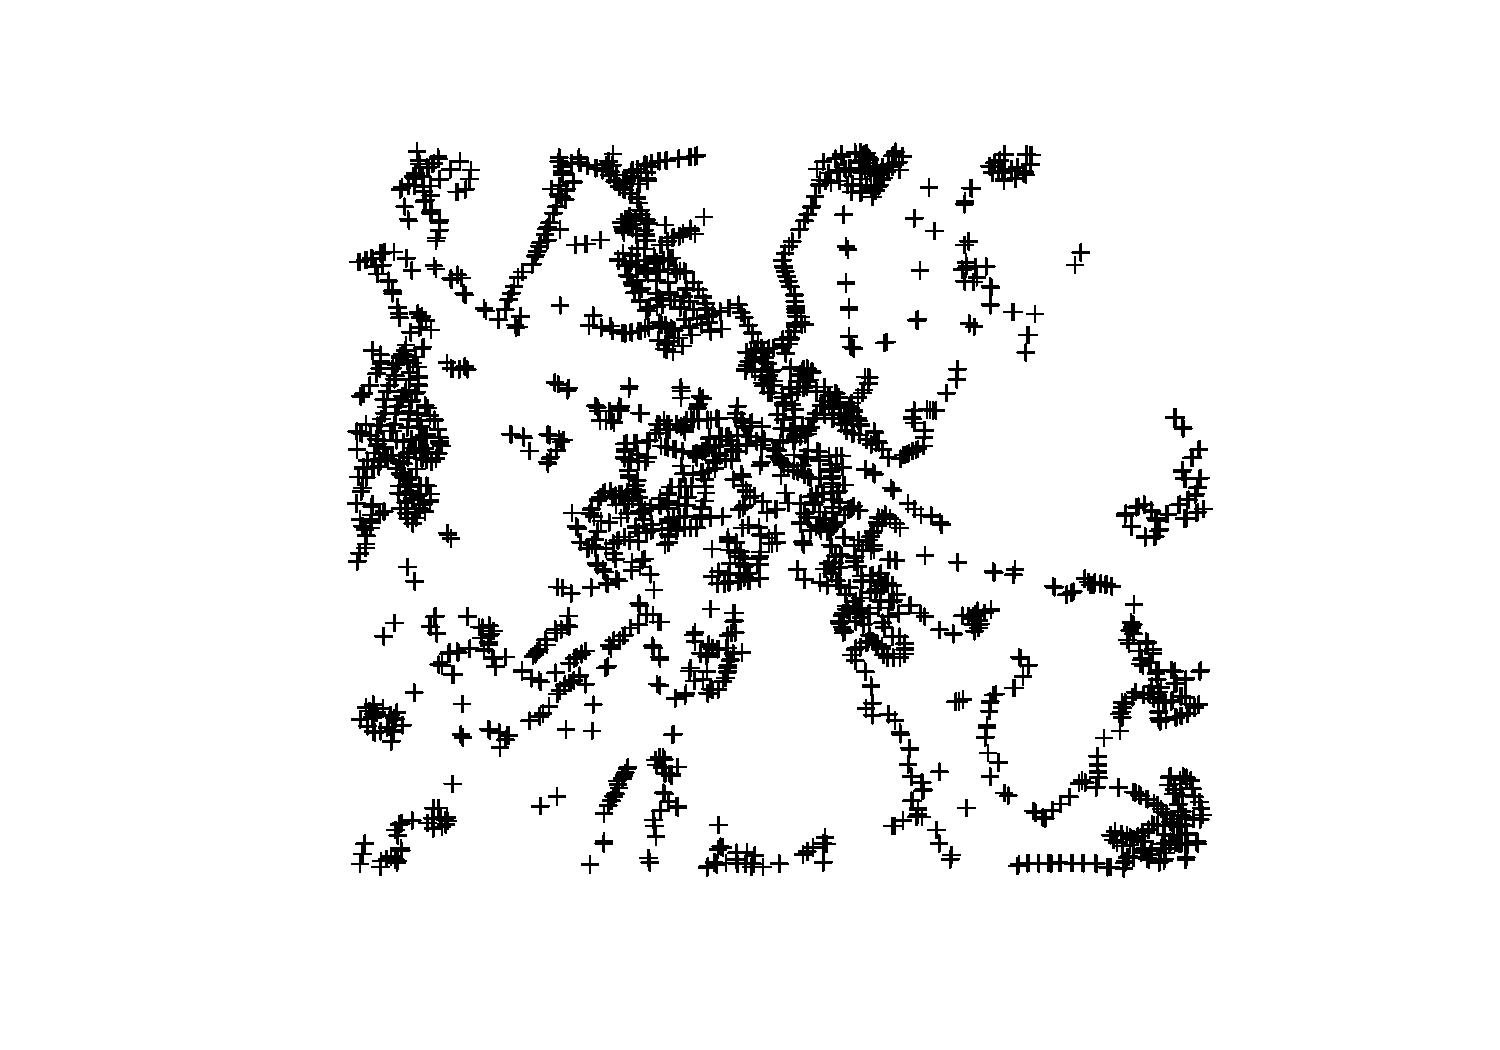
\includegraphics{using_javascript_files/figure-beamer/unnamed-chunk-26-1.pdf}

\end{frame}

\begin{frame}[fragile]{\href{https://cran.r-project.org/web/packages/lawn/index.html}{Das
Paket \texttt{lawn}}}

\begin{itemize}
\item
  \href{https://cran.r-project.org/web/packages/lawn/vignettes/lawn_vignette.html}{\textbf{Vignette}}
  für das Paket \texttt{lawn}
\item
  Mit dem Paket \texttt{lawn} kann die Javascript-Bibliothek turf.js in
  R eingebunden werden.
\item
  Weitere genutzte Javascript Bibliotheken (geojson-random und
  geojsonhint), werden verwendet um GeoJSON-Objekte zufällig zu erzeugen
  bzw. um die GeoJSON Objekte einzufärben.
\end{itemize}

\begin{Shaded}
\begin{Highlighting}[]
\KeywordTok{install.packages}\NormalTok{(}\StringTok{"lawn"}\NormalTok{)}
\KeywordTok{citation}\NormalTok{(}\StringTok{"lawn"}\NormalTok{)}
\end{Highlighting}
\end{Shaded}

\begin{Shaded}
\begin{Highlighting}[]
\KeywordTok{library}\NormalTok{(lawn)}
\end{Highlighting}
\end{Shaded}

\end{frame}

\begin{frame}[fragile]{Ein zufälliges Beispiel Objekt erstellen}

\begin{itemize}
\tightlist
\item
  Mit der Funktion \texttt{gr\_polygon} kann ein Beispielobjekt erzeugt
  werden.
\item
  Anschließend kann man sich das Objekt mit der generischen Funktion
  \texttt{view} plotten.
\end{itemize}

\begin{Shaded}
\begin{Highlighting}[]
\NormalTok{a <-}\StringTok{ }\KeywordTok{gr_polygon}\NormalTok{(}\DataTypeTok{n =} \DecValTok{1}\NormalTok{, }\DataTypeTok{vertices =} \DecValTok{5}\NormalTok{, }\DataTypeTok{max_radial_length =} \DecValTok{5}\NormalTok{)}
\KeywordTok{view}\NormalTok{(a)}
\end{Highlighting}
\end{Shaded}

\begin{Shaded}
\begin{Highlighting}[]
\NormalTok{b <-}\StringTok{ }\KeywordTok{gr_polygon}\NormalTok{(}\DataTypeTok{n =} \DecValTok{1}\NormalTok{)}
\KeywordTok{view}\NormalTok{(b)}
\end{Highlighting}
\end{Shaded}

\end{frame}

\begin{frame}[fragile]{Interaktive Deutschland Karte}

\begin{Shaded}
\begin{Highlighting}[]
\NormalTok{gcs <-}\StringTok{ }\NormalTok{geojsonio}\OperatorTok{::}\KeywordTok{geojson_read}\NormalTok{(}\StringTok{"../data/ddat.geojson"}\NormalTok{)}
\KeywordTok{view}\NormalTok{(gcs)}
\end{Highlighting}
\end{Shaded}

\end{frame}

\begin{frame}[fragile]{Das Paket \texttt{jsonlite}}

\begin{itemize}
\tightlist
\item
  A Robust, High Performance JSON Parser and Generator for R
\end{itemize}

\begin{Shaded}
\begin{Highlighting}[]
\KeywordTok{library}\NormalTok{(jsonlite)}
\NormalTok{geoc <-}\StringTok{ }\KeywordTok{read_json}\NormalTok{(}\StringTok{"../data/ddat.geojson"}\NormalTok{)}
\end{Highlighting}
\end{Shaded}

\begin{Shaded}
\begin{Highlighting}[]
\KeywordTok{citation}\NormalTok{(}\StringTok{"jsonlite"}\NormalTok{)}
\end{Highlighting}
\end{Shaded}

\begin{verbatim}
## 
## To cite jsonlite in publications use:
## 
##   Jeroen Ooms (2014). The jsonlite Package: A Practical and
##   Consistent Mapping Between JSON Data and R Objects.
##   arXiv:1403.2805 [stat.CO] URL https://arxiv.org/abs/1403.2805.
## 
## A BibTeX entry for LaTeX users is
## 
##   @Article{,
##     title = {The jsonlite Package: A Practical and Consistent Mapping Between JSON Data and R Objects},
##     author = {Jeroen Ooms},
##     journal = {arXiv:1403.2805 [stat.CO]},
##     year = {2014},
##     url = {https://arxiv.org/abs/1403.2805},
##   }
\end{verbatim}

\end{frame}

\begin{frame}[fragile]{Das Paket \texttt{RJSONIO}}

\begin{Shaded}
\begin{Highlighting}[]
\KeywordTok{library}\NormalTok{(}\StringTok{"RJSONIO"}\NormalTok{)}
\NormalTok{con <-}\StringTok{ }\KeywordTok{url}\NormalTok{(}\StringTok{"http://nominatim.openstreetmap.org/search?format=json&}
\StringTok{addressdetails=1&extratags=1&q=Amsterdam+Niederlande+Rozengracht+1"}\NormalTok{)}
\NormalTok{geoc <-}\StringTok{ }\KeywordTok{fromJSON}\NormalTok{(}\KeywordTok{paste}\NormalTok{(}\KeywordTok{readLines}\NormalTok{(con,}\DataTypeTok{warn=}\NormalTok{F), }
                       \DataTypeTok{collapse =} \StringTok{''}\NormalTok{))}
\KeywordTok{close}\NormalTok{(con)}
\end{Highlighting}
\end{Shaded}

\end{frame}

\begin{frame}{Links und Quellen}

\begin{itemize}
\item
  \href{http://www.r-bloggers.com/the-leaflet-package-for-online-mapping-in-r/}{Rbloggers
  Artikel zu Leaflet}
\item
  \href{https://rstudio.github.io/leaflet/}{Einführung in Leaflet für R}
\item
  \href{https://blog.hwr-berlin.de/codeandstats/category/scientific-software/r/}{Offline
  Karten mit RgoogleMaps und leaflet}
\item
  \href{https://github.com/ropensci/lawn}{github Ordner für das lwan
  Paket}
\end{itemize}

\end{frame}

\end{document}
